\scanpage{33}\mspage{32.}
% Provisional main reading; all revisions remain subject to independent-reader comparison.
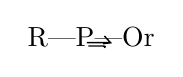
\begin{tikzpicture}[baseline=(old.base),x=1em,y=1em]
\node[inner sep=0pt] (old) at (0,0) {\deleted{\unsure{R|P|Or}}};
\draw[line width=.5pt] (-.15,-.2)--(.7,-.2)--(.48,.04);
\draw[line width=.5pt] (.7,-.2)--(.43,-.24);
\draw[line width=.5pt] (-.10,-.32)--(.40,-.32)..controls(.52,-.32)and(.54,-.35)..(.48,-.39);
\end{tikzpicture}
1°) $F\setminus G\subset F'\setminus G'$ i.e. Tout $A\in F\setminus G$ est $\notin G'$. En effet, si on avait $A\in G'$, on aurait $|A|\subset|G'|=|G|$ donc \deleted{$A\in$} (comme $G\leq F$) $A\in G$.

% @ vertical left margin, with long thin separation stroke
\margin{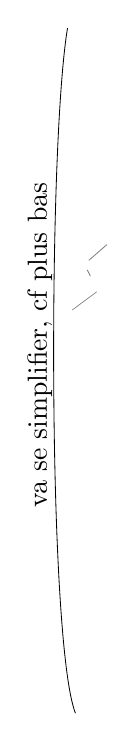
\begin{tikzpicture}
\node[rotate=90,anchor=west,inner sep=0pt] at (0,-1.8) {va se simplifier, cf plus bas};
\draw[line width=.3pt] (.35,4.3)..controls(.1,2.8)and(.1,-3.5)..(.45,-4.4);
% Two faint stroke clusters to the right of the rule, beside Je dis.
\draw[gray,line width=.3pt] (.62,1.35)--(.85,1.55);
\draw[gray,line width=.3pt] (.60,1.23)--(.64,1.15);
\draw[gray,line width=.25pt] (.41,.72)--(.72,.95);
\end{tikzpicture}}

2°) $F'\setminus G'\subset F\setminus G$ Soit $A'\in F'\setminus G'$, prouvons $A'\in F\setminus G$, et d'abord $A'\in F$. \deleted{On a} Soit $A$ le plus petit él. de $F^{A'}$ donc
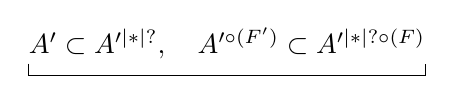
\begin{tikzpicture}[baseline=(f.base)]
\node[inner sep=0pt] (f) at (0,0) {$A'\subset A^{\deleted{\unsure{\prime|\ast|?}}},\quad A'^{\circ(F')}\subset A^{\deleted{\unsure{\prime|\ast|?}}\unsure{\circ(F)}}$};
\draw[line width=.4pt] ([yshift=-.05cm]f.south west)--([yshift=-.2cm]f.south west)--([yshift=-.2cm]f.south east)--([yshift=-.05cm]f.south east);
\end{tikzpicture}
prouvons que $A'\unsure{\deleted{\unsure{\in|\subset}}=|\in}A$ (d'où $A\in F$). \deleted{On a}

Je dis que $A\in F\setminus G$ i.e. $A\notin G$, sinon on aurait $A\subset|G|=|G'|$ donc $A'\in G'$ puisque $A'\in F'$ et $G'\leq F'$, absurde. \deleted{Mais} Donc $A\in F\setminus G$, donc $A\in F'$, \deleted{et} Il en résulte que $A^{\circ(F)}=A^{\circ(F')}$
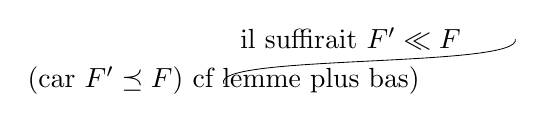
\begin{tikzpicture}[baseline=(lemma.base)]
\node[anchor=base west,inner sep=0pt] (lemma) at (0,0) {(car $F'\preceq F$\deleted{)} cf lemme plus bas)};
\node[anchor=base west,inner sep=0pt] at (2.7,.5) {\inserted{il suffirait $F'\ll F$}};
\draw[line width=.3pt] (2.5,.05)..controls(2.3,.43)and(6.3,.25)..(6.2,.62);
\end{tikzpicture}
et \unsure{\uline{bien}|\deleted{bien}} \deleted{$\unsure{F|\in|\exists}$} $A,A'\in F'$ tels que $A'^{\circ(F')}\subset A^{\circ(F')}$, ce qui prouve $A=A'$.

Donc \unsure{on a} prouvé que $\deleted{\unsure{F|A}}A'\in F'\setminus G'\Rightarrow A'\in F$. Prouvons qu'on a $A'\notin G$ (d'où $A'\in F\setminus G$\deleted{)}, qed). Sinon on aurait $A'\in G$, on aurait $A'\subset |G|=|G'|$, d'où
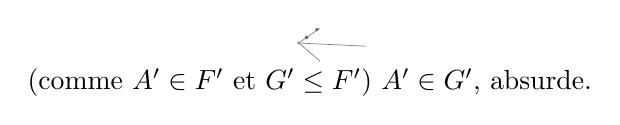
\begin{tikzpicture}[baseline=(last.base)]
\node[anchor=base west,inner sep=0pt] (last) at (0,0) {(comme $A'\in F'$ et $G'\leq F'$) $A'\in G'$, absurde.};
% Separate pale mark above et: reproduced without assigning a mathematical role.
\draw[gray,line width=.25pt] (4.3,.55)--(3.45,.59)--(3.72,.78);
\draw[gray,line width=.25pt] (3.45,.59)--(3.72,.36);
\fill[black!60] (3.55,.66) circle (.025);
\fill[black!60] (3.68,.76) circle (.025);
\fill[black!45] (3.45,.59) circle (.02);
\end{tikzpicture}

% @ abandoned argument, with upper insertion and five oblique strokes
\figure{\begin{tikzpicture}
\node[anchor=base west,inner sep=0pt] at (2.8,.55) {\deleted{\inserted{On suppose b) i.e. $\varphi$ induit $F'\setminus G'\overset{\sim}{\longrightarrow}F\setminus G$}}};
\node[anchor=base west,inner sep=0pt] at (0,0) {\deleted{b) $\Rightarrow$ c) Soit $A\in F\setminus G$, prouvons que}};
\node[anchor=base west,inner sep=0pt] at (0,-.75) {\deleted{$A^{\circ(F)}$ est une \uline{strate ouverte \deleted{dans \unsure{la}} de} $F'$. Soit}};
\node[anchor=base west,inner sep=0pt] at (0,-1.5) {\deleted{$A'\in F'\setminus G'$ l'unique élément \deleted{de} tel que $\varphi(A')=A$.}};
% The final uncrossed baseline may share the paragraph-level cancellation.
\node[anchor=base west,inner sep=0pt] at (0,-2.25) {\unsure{\deleted{Prouvons $A'^{\circ(F')}=A^{\circ(F)}$.}}};
\draw[line width=.3pt] (2.65,-.2)..controls(2.4,.35)and(11.7,.2)..(11.9,.62);
\draw[line width=.4pt] (.15,-1.7)--(1.65,.45);
\draw[line width=.4pt] (2.5,-1.8)--(4.2,.55);
\draw[line width=.4pt] (5.4,-1.7)--(7.1,.6);
\draw[line width=.4pt] (8.1,-1.65)--(9.7,.55);
\draw[line width=.4pt] (10.4,-1.65)--(11.7,.4);
\end{tikzpicture}}

b $\Longleftrightarrow$ c \deleted{Posons} On a $|F|\setminus|G|=|F'|\setminus|G'|$, soit $U$, Posons $F\setminus G=I^{\unsure{k|\ast|+}},\ F'\deleted{\unsure{\times|\setminus}}\unsure{\setminus}G'=I'^{\unsure{k|\ast|+}}$ (parties ouvertes des ens d'indices ordonnés $\unsure{I|\vec I}$, \deleted{$\unsure{A|\Delta}$} $(=F)$, $I'(=F')$. On a
